\chapter{Linear and Logistic Regression via grad descent}
\label{ch-linear-reg-bnets}
%\begin{refsection}

\begin{figure}[h!]
\centering
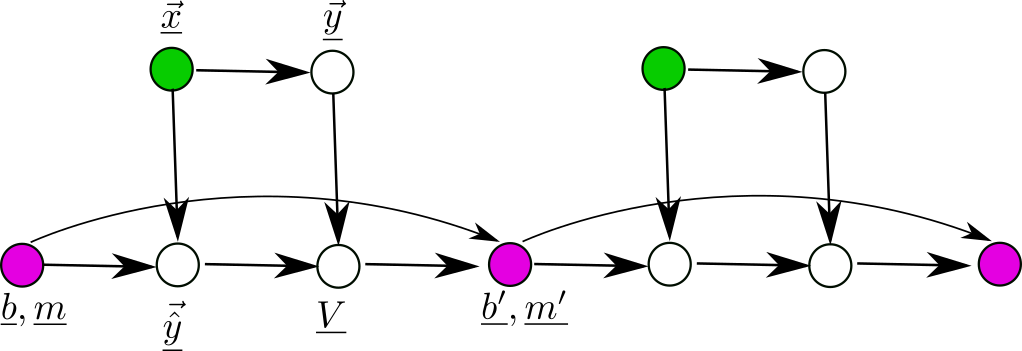
\includegraphics[width=5in]{linear-reg-bnets/linreg.png}
\caption{Linear Regression}
\label{fig-linreg}
\end{figure}

\begin{figure}[h!]
\centering
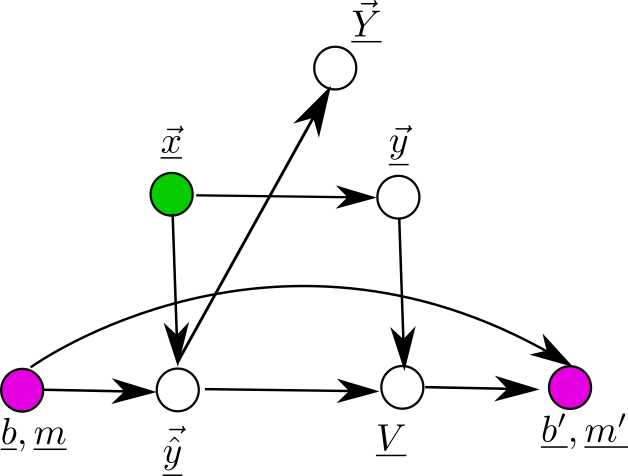
\includegraphics[width=3in]{linear-reg-bnets/linreg-emul.png}
\caption{Bnet of Fig.\ref{fig-linreg}  with new $\vec{\ul{Y}}$ node.}\label{fig-linreg-emul}
\end{figure}



Estimators $\haty$ for linear and logistic regression.
\begin{itemize}
\item

\textbf{Linear Regression:} $y\in \RR$.
Note $\haty\in \RR$. $(x,\haty(x))$ is
the graph
of a straight line
with y-intercept $b$ and slope $m$.
\beq
\haty(x;b, m)= b + mx
\eeq

\item
\textbf{Logistic Regression:} $y\in\{0, 1\}$. Note $\haty\in [0,1]$. $
(x,\haty(x))$ is the graph
of a sigmoid.
 Often in literature, $b,m$ are replaced by $\beta_0, \beta_1$.
\beq
\haty(x;b, m)=\smoid(b + m x)
\eeq
\end{itemize}

Define
\beq
V(b, m)=\sum_{x,y}P(x,y)| y-\haty(x;b, m)|^2
\;.\label{eq-norm-cost}
\eeq
We want to minimize $V(b,m)$ (called a cost or loss function) wrt $b$ and $m$.


The TPMs, printed in blue, for the
Bnet Fig.\ref{fig-linreg}, are as follows.

\beq\color{blue}
P(b,m) \text{ = given}
\eeq
The first time it is used,
$(b,m)$ is arbitrary.
After the first time, it is determined
by previous stage.

Let
\beq
P_{\rvx, \rvy}(x,y)=
\frac{1}{nsam(\vecx)}
\sum_\s \indi(x=x^\s, y=y^\s)
\;.
\eeq

\beq\color{blue}
P(\vecx)=\prod_\s P(x^\s)
\eeq

\beq\color{blue}
P(\vecy|\vecx)=\prod_\s P(y^\s\cond x^\s)
\eeq

\beq\color{blue}
P(\vec{\haty}|\vecx, b, m)=\prod_\s \delta(\haty^\s, \haty(x^\s,b,m))
\label{eq-replace1}
\eeq

\beq\color{blue}
P(V|\vec{\haty}, \vecy)=
\delta(V, \frac{1}{nsam(\vecx)}\sum_\s |y^\s-\haty^\s|^2)
\label{eq-replace2}
\eeq
Let $\eta_b, \eta_m>0$.
For $x=b,m$, if
$x'-x=\Delta x =
-\eta\frac{\partial V}{\partial x}$,
 then $\Delta V\approx
 \frac{-1}{\eta}(\Delta x)^2   \leq 0$
 for $\eta>0$. This is called \qt{gradient descent}.
\beq\color{blue}
P(b'|V, b)=\delta(b', b-\eta_b\partial_b V)
\eeq
\beq\color{blue}
P(m'|V, m)=\delta(m', m-\eta_m\partial_m V)
\eeq


\section{Generalization to
$x$ with multiple
components (features)}

 Suppose that for each sample $\s$,
instead of $x^\s$ being a scalar,
it has $n$ components called features:

 \beq
x^\s = (x_0^\s, x_1^\s, x_2^\s , \ldots x_{n-1}^\s)
\;.\eeq

Slope $m$ is replaced by weights

\beq
w = (w_0, w_1, w_3, , \ldots, w_{n-1})
\;,\eeq
and the product of 2  scalars $mx^\s$ is replaced by the inner vector product $w^Tx^\s$.

\section{Alternative $V(b,m)$
 for logistic regression}

For logistic regression, since $y^\s\in \{0,1\}$
 and $\haty^\s\in [0,1]$ are both
in the interval $[0,1]$, they can
be interpreted as probabilities. Define
probability distributions $p^\s(x)$ and
$\HAT{p}^\s(x)$ for $x\in \{0,1\}$ by
\beq
p^\s(1)=y^\s,\;\;\; p^\s(0)=1-y^\s
\eeq

\beq
\HAT{p}^\s(1)=\haty^\s,\;\;\; \HAT{p}^\s(0)=1-\haty^\s
\eeq
Then for logistic regression, the following 2 cost functions $V(b,m)$
can be used as alternatives to the cost function Eq.(\ref{eq-norm-cost}) previously given.

\beq
V(b, m)= \frac{1}{nsam(\vecx)}\sum_\s
 D_{KL}(p^\s\parallel \HAT{p}^\s)
\eeq

and

\beqa
V(b, m)&=&\frac{1}{nsam(\vecx)} \sum_\s
CE(p^\s\parallel\HAT{p}^\s)\\
&=& \frac{-1}{nsam(\vecx)}\sum_\s \left\{
y^\s\ln \haty^\s +
(1-y^\s)\ln (1- \haty^\s)\right\}\\
&=&
\frac{-1}{nsam(\vecx)}\sum_\s
\ln \left\{(\haty^\s)^{y^\s}
(1- \haty^\s)^{(1-y^\s)}\right\}\\
&=&
\frac{-1}{nsam(\vecx)}\sum_\s
\ln P(\ul{Y}=y^\s\cond \haty=\haty^\s)\\
&=&
-\sum_{x,y} P(x, y)
\ln P(\ul{Y}=y|\haty=\haty(x,b,m))
\eeqa

Above, we used
\beq
P(\ul{Y}=Y|\haty) = \haty^{Y}
[1-\haty]^{1-Y}
\eeq
for $Y\in S_{\ul{Y}}=\{0,1\}$. (Bernoulli distribution).

There is no node corresponding to $\ul{Y}$
in the Bnet of Fig.\ref{fig-linreg}.
Fig.\ref{fig-linreg-emul} shows a new Bnet
that has a new node called $\vec{\ul{Y}}$
compared to the Bnet of Fig.\ref{fig-linreg}.
One defines the TPMs
for all nodes of Fig.\ref{fig-linreg-emul}
except $\vec{\ul{Y}}$ and $\ul{V}$ the same
as for Fig.\ref{fig-linreg}. For $\vec{\ul{Y}}$
and $\ul{V}$, one defines

\beq\color{blue}
P(Y^\s\cond \vec{\haty})=
P(\ul{Y}=Y^\s\cond \haty^\s)
\eeq

\beq\color{blue}
P(V|\vec{Y}, \vecy)=
\delta(V, \frac{-1}{nsam(\vec{x})}\ln  L)
\;,
\eeq
where $ L =\prod_\s P(\ul{Y}=y^\s\cond \haty^\s )$=likelihood.
